\chapter{Analyse de l’\'existant}

\section{Existant Organisationnel}

\section{Processus strat\'egiques}

\section{Existant informatique}

\subsection{Cartographie applicative}

\begin{figure}[h]
    \centering
    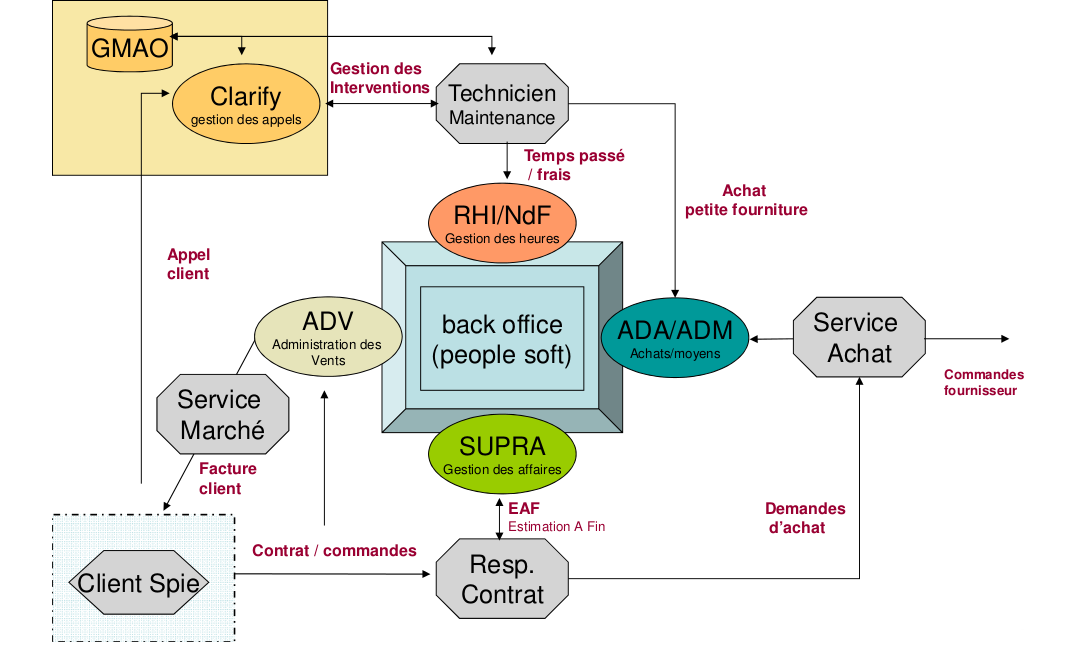
\includegraphics[width=140mm]{./images/cartographie_applicative.png}
    \caption{Cartographie applicative du système de gestion de contrats de maintenance de SPIE}
    \label{diagram:carto_app}
\end{figure}

\subsection{Description de l'architecture applicative}

Le système de gestion de contrats utilise 5 applications différentes :

%ADV : Administration des ventes
%ADA : Administration des achats
%ADM : Administration des moyens
%RHI : Relevé Hebdomadaire Individuel (Temps d'intervention des techniciens sur site)
%NdF : Note de Frais
%EAF : Estimation à fin (reste à faire)
%Clarify : Application de gestion des appels clients
%SUPRA : Application de gestion et suivi des affaires

\begin{itemize}
\item Clarify : Gestion des appels clients
\item RHI/NdF : Relevé Hebdomadaire Individuel / Note de frais
\item ADV : Administration des Ventes
\item ADA/ADM : Administration des Achats / Administration des moyens
\item SUPRA : Gestion et suivi des affaires
\end{itemize}


\subsubsection{Clarify}

Clarify est un outils de gestion des appels des clients. Lorsqu'un client appelle,  %TODO

\subsubsection{RHI/NdF}
\subsubsection{ADV}
\subsubsection{ADA/ADM}
\subsubsection{SUPRA}

\subsection{Améliorations possibles}

Nous pourrions penser à ajouter un dispositif nomade que les techniciens de SPIE puissent emporter avec eux lors de leurs opérations de maintenance. 
Ces appareils leurs permettraient par exemple :

\begin{itemize}
\item de se tenir à jour en temps réels de l'évolution des contrats
\item de remonter des problèmes rencontrés lors d'une opération de façon immédiate
\item d'enregistrer les nouvelles demandes du clients.
\item d'enregistrer les notes de frais
\item de rapporter leur temps d'intervention sur un site
\end{itemize}

\section{Dysfonctionnements}
